\begin{figure*}[t]
\centering
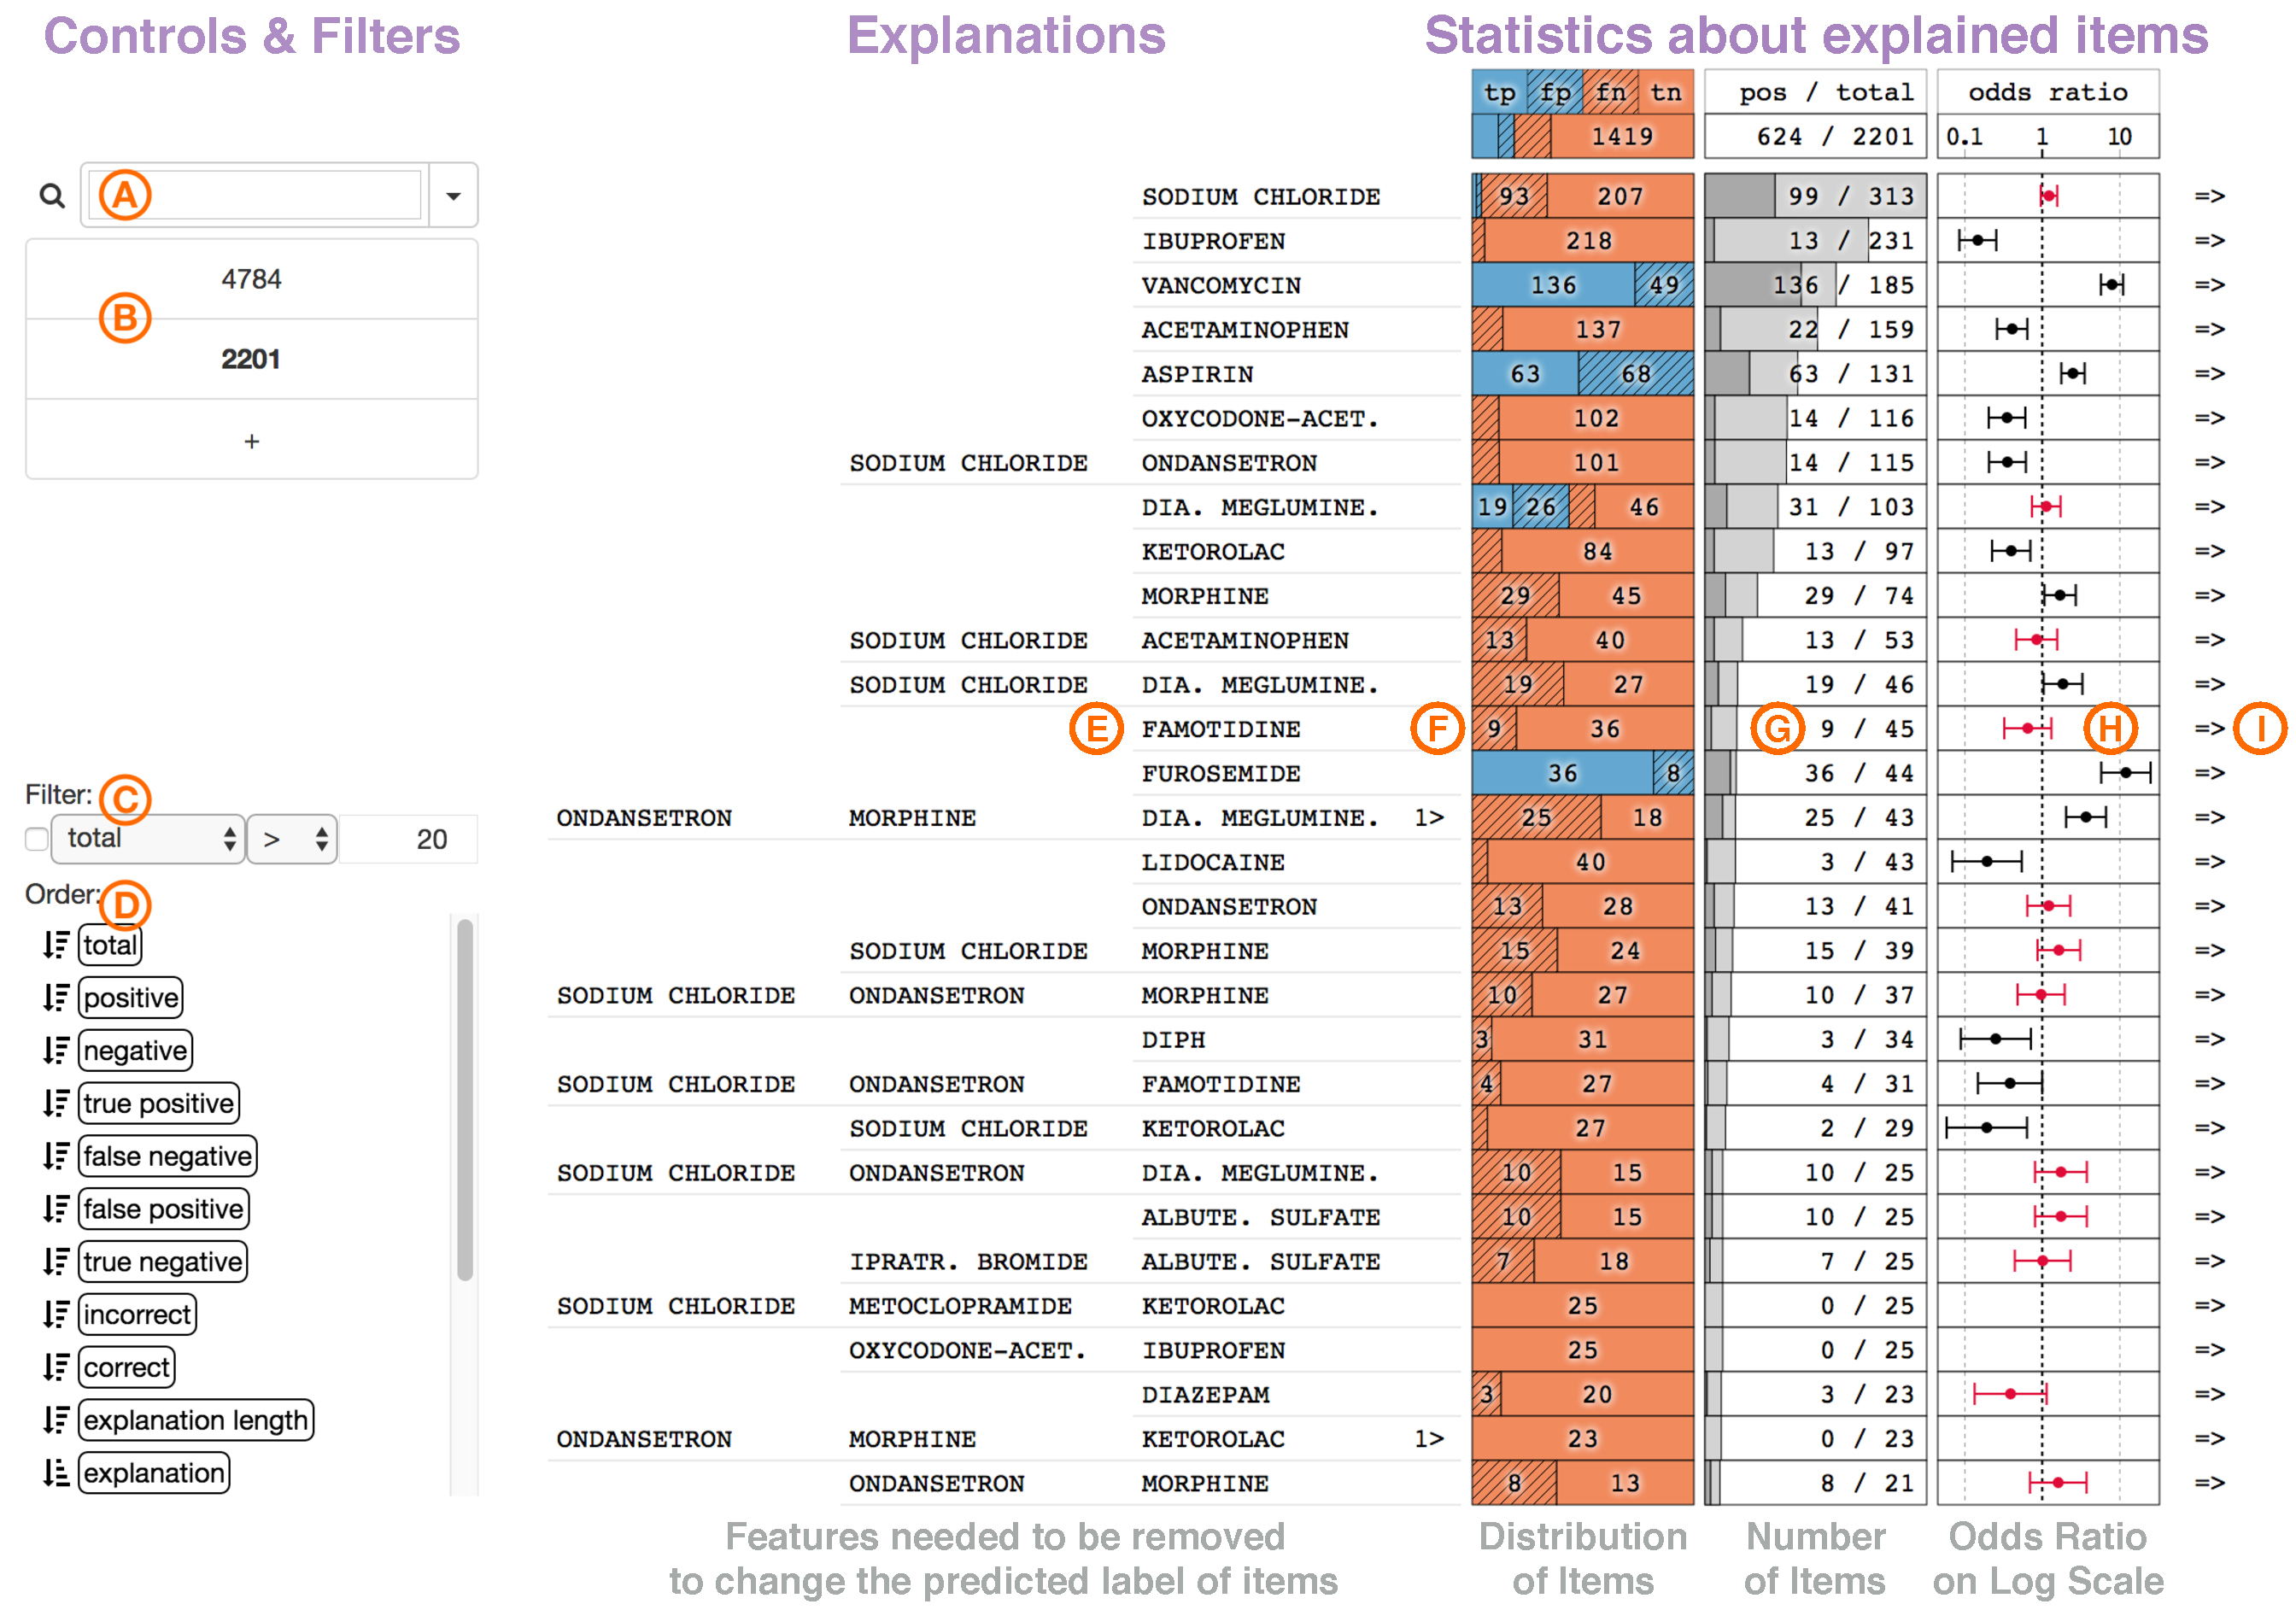
\includegraphics[width=0.8\linewidth]{explainer/controlexplain}%
\raisebox{2.05em}{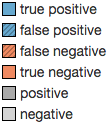
\includegraphics[height=6.9em]{explainer/iamlegend}}
\vspace{-3mm}
\caption{
In the \textbf{\tabB} each row represents a group of data items explained by a set of features (E).
An indicator is shown for explanations longer than 3 features.
Column (F) shows the distribution of true / false positive / negative data items within the group.
Colors show the predicted label (``blue" for positive and ``orange" for negative) and a hatching pattern indicates incorrect predictions.
Column (G) shows the number of items captured by the explanation.
The bars are relative to the size of the largest explanation.
Column (H) shows the odds ratio of the group on a logarithmic scale.
Whiskers show the confidence interval.
The arrows on the right (I) navigate to the \tabC focusing on the given explanation. The controls of the \tabB are shown on the left.
The first entry of the list of filtered data items (B) represents the full dataset and following entries show sizes after filter steps are applied.
The ``+" creates a new filter according to the current selection of explanations.
Explanations can be selected satisfying a condition (C) or by searching for features in the search box (A).
The sort order of explanations is defined by the list at the bottom (D).
}
\vspace{-5mm}
\label{figs:expl_main}
\end{figure*}